
%-------------------------------------------------------------
%			PAGE BUILDER
%-------------------------------------------------------------

\mcchap{Integrazione Page Builder}{cap:pb}

Per passare ad una gestione più semplice delle pagine da parte dei Content
mi è stato chiesto di cercare qualche sistema che permettesse una suddivisione
della pagina in componenti facilmente editabili e riutilizzabili.

Le esigenze principali erano:
\begin{itemize}
\item modificare il contenuto delle componenti da interfaccia grafica e non 
editando il codice HTML.
\item poter creare semplicemente copie delle componenti già create
\item poter spostare le varie componenti con \emph{drag and drop} e avere
feedback visivo immediato della modifica della pagina
\end{itemize}

Per questo mi è stato consigliato di fare una ricerca tra le varie soluzioni disponibli
nella ampia libreria di plugin di Wordpress.


Dopo aver analizzato i vari plugin disponibili è stata individuata una soluzione open source chiamata \emph{Page Builder by
Site Origin}\cite{PB} che soddisfava le esigenze.

\section{Page Builder by Site Origin}

Il plugin \emph{Page Builder} permette la suddivisione della pagina in colonne all'interno delle quali
si possono inserire delle componenti.

Queste componenti possono essere duplicate, modificate aprendo il form della componente e spostate
con drag and drop.


Il vantaggio di questo plugin rispetto ad altri plugin che permettono la suddivisione della pagine è che all'interno delle colonne
oltre a poter inserire delle componenti standard fornite dal plugin si possono anche inserire i Widget di Wordpress.

\section{Widget}
I \emph{Widget} sono delle componenti riutilizzabili che possono essere aggiunte a qualsiasi
tipo di pagina Wordpress. 

Classici esempi di Widget sono le icone per i link ai social network, o un anteprima di un post creato, tuttavia è possibile creare Widget
personalizzati.

Per creare un widget bisogna implementare una sottoclasse di WpWidget\cite{WPWID}
e sovrascrivere il metodo \emph{widget} dove viene restituito il contenuto HTML che la pagina deve restituire quando quel widget viene incluso
e, se si vuole del contenuto dinamico, bisogna sovrascrivere \emph{form} dove viene creato il form HTML che verrà visualizzato dai content per modificare le
parti dinamiche della componenti utilizzato da \emph{innin}.

Le componenti compilate nel form vengono poi utilizzate dal metodo \emph{widget}.


\lstinputlisting[style=customphp, language=Php]{code/exampleWidget.php}
\emph{Una semplice implementazione di un widget che stampa un titolo dinamicamente}


\begin{figure}
  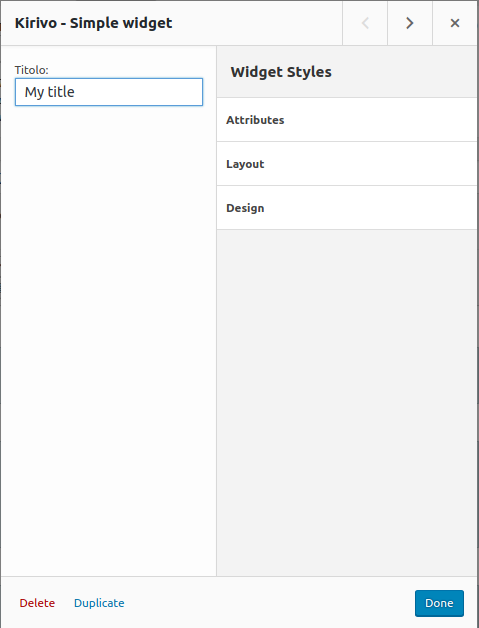
\includegraphics[width=0.6\textwidth]{figure/wid_form.png}
  \caption{Il form che viene visualizzato per modificare i dati del Widget.}
  \label{fig:wform}
\end{figure}
\begin{figure}
  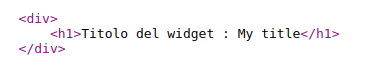
\includegraphics[width=0.7\textwidth]{figure/sourcewid.png}
  \caption{Porzione di sorgente di una pagina che utilizza il widget compilato come in \ref{fig:wform}.}
  \label{fig:wsource}
\end{figure}

\newpage

\section{Inizializzazione}
Per inizializzare i Widget bisogna aggiungere una action\cite{WPACTION}, ovvero un meccanismo offerto da Wordpress per aggiungere dei comportamenti
prestabiliti,  chiamata \emph{init\_widget} dove viene aggiunto ogni Widget creato.

Per far in modo di non dover aggiungere manualmente un Widget al file di inizializzazione ogni volta che se ne crea uno nuovo, è
stato implementato un script di inizializzazione che va all'interno delle cartelle \emph{widget\_orgini} e \emph{widget\_kirivo} e aggiunge tutti
i Widget che trova all'interno di queste cartelle, per individuare un widget allìinterno della cartella viene fatto pattern-matching per i file che terminano con \emph{Widget.php}.

\lstinputlisting[style=customphp, language=Php]{code/intializeWidget.php}
\emph{Il file initialize\_widget.php}

\newpage

\section{Implementazione Widget}
Per implementare i Widget necessari per le Homepage sono state isolate le componenti HTML necessarie e per ognuna
di queste è stato creato un Widget poi , per ognuna di queste è stato create il form per le componenti che potevano essere
modificate dai Content.

Ci sono due categorie principali di widget
\begin{itemize}
\item Widget che non contengono prodotti.
\item Widget che contengono prodotti.
\end{itemize}

Per implementare i Widget che non contengono prodotti è stato messo all'interno del metodo \emph{widget} direttamente
l'HTML di quella componenta con eventuale contenuto dinamico stampato con php.

Per i widget che contengono prodotti invece all'interno di \emph{widget} non è stato inserito il codice HTML con il template
di ogni prodotto ma è stato messo il tag \emph{dynamic} i cui attributi sono popolati dinamicamente in base al contenuto del form.
Una volta che il server Kiruby prende una pagina Wordpress e trova il dynamic tag allora provvede a sostituire il tag con le 'tile'
di tutti i prodotti specificati.
